\documentclass[12pt]{article}

\usepackage{tabularx}
\usepackage[a4paper,margin=2.5cm, bottom=3.5cm]{geometry}
\usepackage{fancyhdr}
\usepackage{listings}
\usepackage{booktabs}
\usepackage{float}
\usepackage{subcaption}
\usepackage{graphicx}
\usepackage{amsmath}
\usepackage{amssymb}
\usepackage{amsthm}
\usepackage{array}
\usepackage[table]{xcolor}
\usepackage{pgfplots}
\usepackage{pgfplotstable}
\usepackage{multirow}
\usepackage{tikz}
\usepackage[hidelinks]{hyperref}
\usepackage{titling}
\pgfplotsset{compat=1.17}

\theoremstyle{definition}
\newtheorem*{example}{Example}
\setlength{\headheight}{40pt}
\setlength{\parindent}{0pt}
\setlength{\parskip}{1ex}
\renewcommand{\headrulewidth}{0pt}

\newcommand{\subfiguresize}{.3\textwidth}
\DeclareMathOperator*{\median}{median}

\DeclareMathOperator*{\biggerforall}{\mbox{\Large $\mathsurround0pt\forall$}} 
\DeclareMathOperator*{\bigforall}{\mbox{\large $\mathsurround0pt\forall$}} 
\DeclareMathOperator*{\biggerexists}{\mbox{\Large $\mathsurround0pt\exists$}} 
\DeclareMathOperator*{\bigexists}{\mbox{\large $\mathsurround0pt\exists$}} 

\lstset {
    captionpos = b,
    basicstyle = \small\ttfamily,
    keywordstyle = \color{blue},
    commentstyle = \color{black!30},
    comment = [l]{//},
    morecomment = [s]{/*}{*/},
    identifierstyle=,
    keywords = {
        let,
        mut,
        for,
        in,
        if,
        else,
        continue,
        break,
        pub,
        struct,
        impl,
        type,
        self,
        Self,
        as,
        u8,u16,u32,u64,
        i8,i16,i32,i64,
        f32,f64,
        usize,
    }
}

\pagestyle{fancy}
\fancyhead{}
\fancyhead[L]{
    \renewcommand{\arraystretch}{1.5}
    \begin{tabularx}{\textwidth}{|X|X|}
        \hline
        \large \bf Image processing & \normalsize \thetitle \\
        \hline
    \end{tabularx}
}
\fancyfoot[C]{\thepage}

\renewcommand{\maketitle}{
    \thispagestyle{plain}
    \renewcommand{\arraystretch}{2}
    \vspace*{-7em}
    \begin{flushleft}
        \begin{tabularx}{0.95\textwidth}{|X|X|}
            \hline
            \bf \large Image Processing                   & \bf \large \thetitle                           \\ \hline
            \multicolumn{2}{|l|}{
                \textbf{Task variant:} Group 1
            }                                                                                               \\ \hline
            \textbf{Day and time:} Mon, 14:00             & \textbf{Full name:} \textsc{Jakub Pawlak}       \\
            \textbf{Academic year:} {2022/23} & \textbf{Full name:} \textsc{Magdalena Paku\l a} \\
            \hline
        \end{tabularx}
    \end{flushleft}
    \vspace{1em}
    \renewcommand{\arraystretch}{1}
}
\graphicspath{{img},{../img}}

\title{Task No.~2}

\begin{document}
\maketitle

\section{Description of the implementation of \texorpdfstring{\\ }{} histogram-based image enhancement method}
Histogram based image enhancements work by assigning new values to the luminosity levels, to match the histogram to some function.
The old luminosities will be denoted as $f$, and the new ones, as $g$.
The histogram of the image is denoted as $H$, and $H(f)$ means the number of pixels with luminosity $f$.
Finally, $n$ will mean the total number of pixels in the image.

\subsection{Mathematical description}

The equation for calculating the new luminosity values were given as:
\begin{equation}
    g(f) = g_{min} +\sqrt{
        2 \alpha^2 \cdot \ln\left[
            \left(
            \frac{1}{n} \sum\limits_{k=0}^f H(k)
            \right)^{-1}
            \right]
    }
    \label{eq:rayleigh-initial}
\end{equation}

We immediately noticed, that the number under the logarithm is a partial sum of the normalized histogram values for luminosities smaller or equal $f$.
We can refactor the equation, by introducing a partial sum function $ps(f)$:
\begin{equation}
    ps(f) = \sum\limits_{k=0}^f H(f)
\end{equation}

Equation (\ref{eq:rayleigh-initial}) then takes form:
\begin{equation}
    g(f) = g_{min} + \sqrt{
        2 \alpha^2 \cdot \ln
        \left(
        \frac{n}{ps(f)}
        \right)}
\end{equation}

Note that,
\(
\bigforall_{f \in \langle f_{min},f_{max}\rangle} : 0 < ps(f) \leq n
\), and $ps(f)$ is monotonically non-decreasing.
That means that $\frac{n}{ps(f)}$ is monotonically non-increasing, and as follows, $g(f)$ is also non-increasing.

However, this is not what we want from image transformation, as it would produce a negative image.
Therefore, we flip the function horizontally, by changing the sign of $ps(f)$, and offsetting it by $n$, to keep the domain the same.

\begin{equation}
    g(f) = g_{min} + \sqrt{
        2 \alpha^2 \cdot \ln
        \left(
        \frac{n}{n - ps(f) + 1}
        \right)}
    \label{eq:rayleigh-corrected}
\end{equation}
Now, as $f$ increases, $g(f)$ will increase as well.

However, the value of $\alpha$ is still unknown.
We know, that the function $g(f)$ should map $f$ to $g$ in such a way, that
$f_{min} \mapsto g_{min}$ and $f_{max} \mapsto g_{max}$.

For the first case:
\(
\lim\limits_{f \to f_{min}} ps(f) = 1
\),which means that
\(
\lim\limits_{f \to f_{min}} g(f) = g_{min}
\) regardless of $\alpha$.

The second case is more interesting:
\begin{align*}
    ps(f_{max}) & = n                \\[1ex]
    g(f_{max})  & = g_{min} + \sqrt{
        2 \alpha^2 \cdot \ln(n)
    }
\end{align*}
Substituting $g(f_{max}) = g_{max}$,
\begin{align}
    g_{max} & = g_{min} + \sqrt{
        2 \alpha^2 \cdot \ln(n)
    }\nonumber                                                                     \\[1ex]
    g_{max} & = g_{min} + \alpha \cdot \sqrt{2\ln(n)} \nonumber                    \\[1ex]
    \alpha  & = \frac{g_{max} - g_{min}}{\sqrt{2\ln(n)}} \label{eq:rayleigh-alpha}
\end{align}

\subsection{Implementation}

We start, by calculating the partial sums of the histogram for each channel:
\begin{lstlisting}
let partial_sums: [[u32; 256]; 3] = {
        let histogram = Histogram::new(image);
        histogram
            .into_iter()
            .map(|h| {
                h.iter()
                    .scan(0u32, |sum, value| {
                        *sum += value;
                        Some(*sum)
                    })
                    .collect()
            })
            .collect::<Vec<[u32; 256]>>()
            .try_into()
            .unwrap()
    };
\end{lstlisting}

\pagebreak[2]
Then, we calculate the image size, and the value of $\alpha$, according to eq. (\ref{eq:rayleigh-alpha})
\begin{lstlisting}
let image_size = image.width() * image.height();
let alpha = (self.gmax - self.gmin) as f64 
    / f64::sqrt(2.0 * f64::ln(image_size as f64));
\end{lstlisting}

\pagebreak[2]
Then, we create the brighness lookup table, according to eq. (\ref{eq:rayleigh-corrected}):
\begin{lstlisting}[basicstyle = \footnotesize\ttfamily]
let mut brightness_lookup = [[0u8; 256]; 3];
for channel in 0..3 {
    for i in 0..256 {
        let partial_sum = partial_sums[channel][i];
        if partial_sum == 0 {
            continue;
        }
        let log_base = 
            image_size as f64 / (image_size - partial_sum + 1) as f64;
        let root_base = 
            2.0 * alpha * alpha * f64::ln(log_base);
        brightness_lookup[channel][i] = 
            self.gmin
            + f64::clamp(
                f64::sqrt(root_base), 
                0.0, 
                (self.gmax - self.gmin) as f64) as u8;
        if partial_sums[channel][i] == image_size {
            break;
        }
    }
}
\end{lstlisting}

Note 2 important things --- the \lstinline{continue} and \lstinline{break} statements inside the loop.
We are interested in filling the lookup table only for values of $f \in \langle f_{min}, f_{max} \rangle$.
Therefore, we check if $ps(f) = 0$. If it is, then $f < f_{min}$, and we need not perform the calculation, so we continue looping
until we encounter some $ps(f) > 0$.

Similarly, we do not need to perform calculations for $f > f_{max}$. We know that $ps(f) = n \Leftrightarrow f \geq f_{max}$,
so if we reach that point, we do not need to perform any calculations for further values of $f$, and can safely break out of the loop.

This is a small optimization compensating for the fact that we cannot create a smaller lookup table, adjusted to the size of $\langle f_{min}, f_{max}\rangle$, because these values are unknown at compile time.

\pagebreak[2]
Finally, we set the new luminosity levels in the image according to the created lookup table:
\begin{lstlisting}
for pixel in image.pixels_mut() {
    for channel in 0..3 {
        let luminosity = pixel[channel];
        let new_luminosity = 
            brightness_lookup[channel][luminosity as usize];
        pixel[channel] = new_luminosity
    }
}
\end{lstlisting}


\section{Image analysis on the basis of the histogram}
\subsection{Implementation}

After conducting an image improvement by using Rayleigh distribution described in the previous section, we could see tremendous differences presented below.

In order to obtain that result, we chose those input numbers as an example.
\begin{align*}
    g_{max} & = 1   \\[1ex]
    g_{max} & = 200
\end{align*}

\subsection{Results}
\begin{figure}[H]\centering
    \begin{subfigure}[t]{\subfiguresize}\centering
        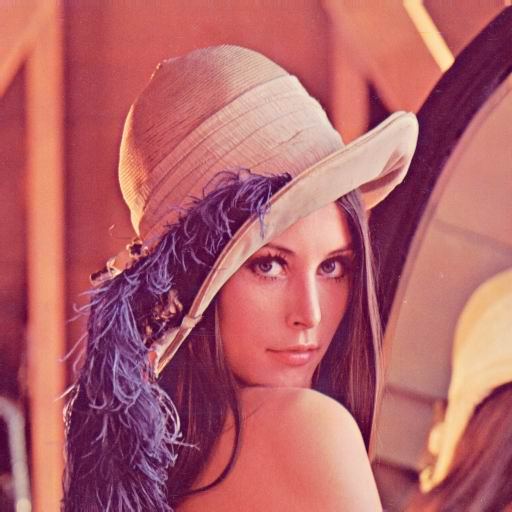
\includegraphics[width=\textwidth]{lenac.png}\\[1ex]
        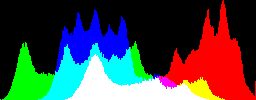
\includegraphics[width=\textwidth]{lena_clear_histogram.png}
        \caption{original}
    \end{subfigure}
    \hspace{.05\textwidth}
    \begin{subfigure}[t]{\subfiguresize}\centering
        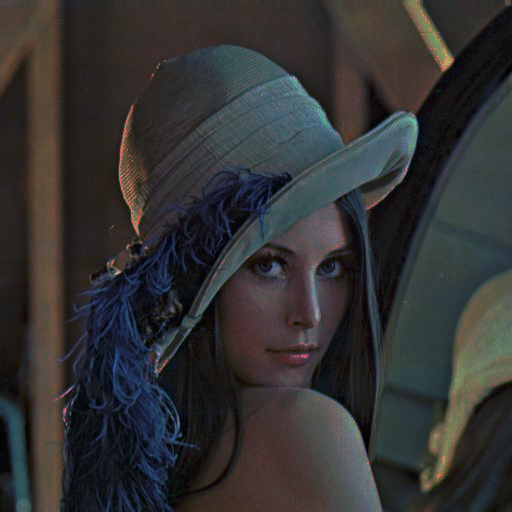
\includegraphics[width=\textwidth]{lena_hraleigh_1_200.png}\\[1ex]
        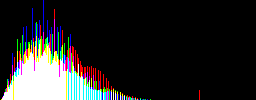
\includegraphics[width=\textwidth]{lena_hraleigh_1_200_histogram.png}
        \caption{modified}
    \end{subfigure}
    \caption{Image before and after Rayleigh distribution correction}
\end{figure}
\subsection{Complex analysis}

As we can see, the difference is huge. the output picture is less red and more neutral for the viewer.
The same difference we can observe on the histogram created on the before and after picture.
While on the original image most of the colors are taking the whole histogram and only part of them are interfering with each other,
on the modified picture almost all the colors are interfering, which resulted in very neutral picture for the viewer, which is not that diverse in colors.
The histogram of the original image has majority of the red channel, which can be seen on the original image as having red undertones.
On the histogram of the modified picture came out with majority of blue tones, which can be clearly seen on the image.
These comparisons can perfectly present a fully working histogram on all the channels at the same time.

\subsection{Characteristics analysis}

In this project we implemented and tested all 8 different characteristics for image transformations which are:
\begin{itemize}
    \item Mean and Variance
          \[
              \bar{b} = \frac{1}{n}\sum\limits_{m=0}^{255} m H(m)
          \]
          \[
              \sigma^2 = \frac{1}{n}
              \sum\limits_{m=0}^{255} \left[ \left(m-\bar{b}\right)^2 H(m) \right]
          \]
    \item Standard deviation and Variation coefficient I
          \[
              \sigma =\sqrt{\sigma^{2}}
          \]
          \[
              b_Z= \frac{\sigma}{\bar{b}}
          \]
    \item Asymmetry coefficient
          \[
              b_S = \frac{1}{n\sigma^3}
              \sum\limits_{m=0}^{255} \left[ \left(m-\bar{b}\right)^3 H(m) \right]
          \]
    \item Flattening coefficient
          \[
              b_K = \frac{1}{n\sigma^3}
              \sum\limits_{m=0}^{255} \left[ \left(m-\bar{b}\right)^4 \cdot H(m)-3 \right]
          \]
    \item Variation coefficient II
          \[
              b_N = \frac{1}{n^2}
              \sum\limits_{m=0}^{255} H(m)^2
          \]
    \item Information source entropy
          \[
              b_I = -\frac{1}{n}
              \sum\limits_{m=0}^{255} \left[ H(m) \cdot \log_2\left(\frac{H(m)}{n}\right) \right]
          \]
\end{itemize}

The result of all of those calculations for the original and modified picture are presented below in the table.

\begin{table}[H]\centering
    \begin{tabular}{l|ccccccccc}
        \toprule
        Operation & $\bar{b}$ & $\sigma^2$ & $\sigma$ & $b_Z$ & $b_S$ & $b_K$ & $b_N$ & $b_I$ \\
        \midrule
        ---       & 128.22    & 3471.79    & 58.99    & 0.46  & 0.22  & 2.11  & 0.005 & 4.368 \\[1ex]
        hraleigh  & 50.87     & 697.74     & 26.42    & 0.52  & 0.74  & 3.90  & 0.003 & 3.035 \\
        \bottomrule
    \end{tabular}
\end{table}

Based on this  comparison we can clearly see differences in these characteristics. 
The ``biggest'' difference we can observe is in variance. 
The rest of the calculations do do not differ so much. 
Those changes in numbers are not the same because of change in pixels and furthermore in histogram. 
Because the luminosity of the pixels in much more neutral, less diverse in comparison to the original image the final result differs.

\section{Description of the linear filter implementation}

\subsection{General formulation}

\subsubsection{Mathematical description}

The linear filter implementation is based on the principle of convolution of the mask $3\times3$ matrix $\mathbf{M}$, with an image fragment of the same size.

Consider a following mask:
\begin{equation}
    \mathbf{M} = \begin{bmatrix}
        a_{0,0} & a_{1,0} & a_{2,0} \\
        a_{0,1} & a_{1,1} & a_{2,1} \\
        a_{0,2} & a_{1,2} & a_{2,2}
    \end{bmatrix}
\end{equation}

Then, for each pixel at coordinates $(x,y)$, we will compute its new value as
\begin{equation}
    g(x,y) = \sum\limits_{i=0}^2 \sum\limits_{j=0}^2 a_{i,j} \cdot f(x + i - 1, y + j - 1)
\end{equation}

Note, that we have to subtract 1, so the pixel $f(x,y)$ will correspond to the center of the $\mathbf{M}$ matrix ($a_{1,1}$).

Important thing, is that for pixels on the edges,
the convolution with $\mathbf{M}$ would require calculating values of pixels outside of the image, which is impossible.
Therefore, for such cases, we assume $g(x,y) = f(x,y)$.

\subsubsection{Implementation}

During the implementation, we noticed that it is sometimes more convenient
to have a separate factor to multiply the matrix with.
For example:
\[
    \mathbf{M} = \begin{pmatrix}
        4 & 2 \\ 2 & 4
    \end{pmatrix} = 2 \begin{pmatrix}
        2 & 1 \\ 1 & 2
    \end{pmatrix}
\]

Moreover, we can factor this value out of the sum, to reduce the number of necessary operations.
Therefore, in our filter settings we store 2 fields: the mask matrix, and the mask scale factor.
When running the program, the user is asked to provide the mask as a command line argument.
They can also provide the optional mask scale (which by default will be set to 1).
This way, it is much more convenient for the user to input masks that have fractional values (like the low-pass filter masks).

Finally, like with all transformations that operate on more than one pixel at a time,
it is necessary to allocate a new image buffer, as to not corrupt the data in the original one.

Having done all this preparation, we are ready to implement the convolution, while remembering to skip the edge pixels:

\pagebreak[3]
\begin{lstlisting}
for (x, y, pixel) in new_image.enumerate_pixels_mut() {
    if is_edge(image, x, y) {
        *pixel = *image.get_pixel(x,y);
        continue;
    }
    for channel in 0..3 {
        let mut sum: f64 = 0.0;
        for i in 0..3 {
            for j in 0..3 {
                sum += (self.mask[j][i])
                    * image.get_pixel(x+i-1, y+j-1)[channel];
            }
        }
        pixel[channel] = (sum * self.mask_scale) as u8;
    }
}
\end{lstlisting}

\paragraph{Important remark}
At the time of writing this report, it was noticed, that although we were supposeed to implement just the low-pass filter,
since the user has the ability to provide any $3\times3$ mask in the command line,
there is nothing stopping them from inputing the mask for e.g.\ line identification or edge sharpening.
Therefore, our implementation actually works not for just low-pass filter, but for all the convolution-based filters with a $3\times3$ mask.

\subsection{With optimization}

\subsubsection{Reasoning}

Looking at the unoptimized implementation of the filter, it was difficult to find the ways of further optimization.
The extraction of the scale factor, already reduced the number of multiplications.
We could optimize the first low-pass filter mask, as it has all 1's in the mask, which would further reduce the number of multiplications,
However, we do not think that it would give such a great performance boost.
We could also, utilize the fact, that the mastrix size is constant, and eliminate the for loops, adding the values manually, since there are only 9 of them.
This would eliminate unnecessary bounds checks on the loop indexes.
However, since the loop ranges are a compile-time constans, the compiler would already perform this optimization (we checked both options and looked at the decompiled code).
Moreover, this could prevent the compiler from doing optimizations specific for loops, such as loop vectorization.

Therefore, we decided to take a completely different approach, and instead of changing the code, we changed the processing unit.
Instead of doing the computations on the \textsc{cpu}, which does the operations sequentially (except some optimizations utilizing the \textsc{simd} instructions),
we moved the computation to the \textsc{gpu}, which is much better at performing simple calculations in parallel.
Since we create the new image buffer, the original image would be read only, and each compute kernel would write to only one pixel of the output image,
this soulution will have no race conditions and be safe to implement as a parallel computation.

\subsubsection{Implementation}
The optimized version would be implemented similarly to the \textsc{gpu}-accelerated filters from the previous task.
We would use Vulkan API to run a compute shader containing the convolution code.

We set the working group size to $16\times16$ pixels, as it is a standard size for processing images,
and we found it to work quite well during previous implementations.
We will provide the shader with the mask as a push constant, so \emph{the optimized version will also work for any $3\times3$ mask}.

\begin{lstlisting}[
    basicstyle=\footnotesize\ttfamily,
    morekeywords={
        float,
        layout,
        in,
        uniform,
        readonly,
        writeonly,
        image2D
    }
]
layout (local_size_x=16, local_size_y=16, local_size_z=1) in;

layout (push_constant) uniform PushConstantData {
        float[9] mask;
} dat;

layout (set=0, binding=0, rgba8) uniform readonly image2D inImg;
layout (set=0, binding=1, rgba8) uniform writeonly image2D outImg;
\end{lstlisting}

The shader will convert the mask to \lstinline{mat3}, which is a builtin type representing a $3\times3$ matrix.
Then, it will collect the luminosity values of the neighboring pixels, also to \lstinline{mat3}.

Finally, it will compute the hadamard product of the 2 matrices using a built-in function \lstinline{matrixCompMult()} (\href{https://registry.khronos.org/OpenGL-Refpages/gl4/html/matrixCompMult.xhtml}{see documentation}).
The final result is the sum of all the elements of the resulting matrix.

\begin{lstlisting}[
    language=C++,
    morekeywords={
        vec3,
        ivec2,
        mat3
    }
]
vec3 convolution(mat3 mask, ivec2 xy)
{
    vec3 pixel;

    // Extract a 3x3 region centered in xy
    mat3[3] region = region3x3(xy);

    // for each color channel of region
    for (int i = 0; i < 3; i++)
    {
        mat3 rc = region[i];
        mat3 c = matrixCompMult(mask, rc);
        // add each component of matrix
        float r =  c[0][0] + c[1][0] + c[2][0]
                 + c[0][1] + c[1][1] + c[2][1]
                 + c[0][2] + c[1][2] + c[2][2];

        pixel[i] = r;
    }

    return pixel;
}
\end{lstlisting}

\subsection{Time comparison}

For greater reliability, we run the tests on the bigger image size ($2560 \times 2560$).
Each implementation was run 3 times, and the average execution time was calculated. The results are shown in table \ref{tab:lowpass-execution-time}.

\begin{table}[ht]\centering
    \begin{tabular}{ccc}
        \toprule
        Test n\textsuperscript{\underline{o}} & unoptimized & optimized \\\midrule
        1                                     & 12.983      & 3.555     \\
        2                                     & 12.996      & 3.465     \\
        3                                     & 12.975      & 3.453     \\\midrule
        \bf avg.                              & 12.985      & 3.491     \\
        \bottomrule
    \end{tabular}
    \caption{Results of testing the execution times of unoptimized and optimized versions of low-pass filter.
        The time values are given in seconds.}
    \label{tab:lowpass-execution-time}
\end{table}

As we can see, there is a clear difference in the execution times.
The standard version took almost 13s to execute, while its optimized counterpart performed in less than 3.5 seconds.
This is a huge increase in the execution speed; the optimized version is over 370\% faster than the standard one.

\section{Analysis of the filtering results (linear filter)}

We run the low-pass filter with the 3 masks given in the instruction:
\begin{equation*}
    \mathbf{M}_1 = \frac{1}{9}\begin{bmatrix}
        1 & 1 & 1 \\
        1 & 1 & 1 \\
        1 & 1 & 1
    \end{bmatrix}
    \qquad
    \mathbf{M}_2 = \frac{1}{10}\begin{bmatrix}
        1 & 1 & 1 \\
        1 & 2 & 1 \\
        1 & 1 & 1
    \end{bmatrix}
    \qquad
    \mathbf{M}_3 = \frac{1}{16}\begin{bmatrix}
        1 & 2 & 1 \\
        2 & 4 & 2 \\
        1 & 2 & 1
    \end{bmatrix}
\end{equation*}

The results are presented on fig. \ref{fig:lowpass-results-original}.

\begin{figure}[ht]\centering
    \begin{subfigure}[t]{.4\textwidth}
        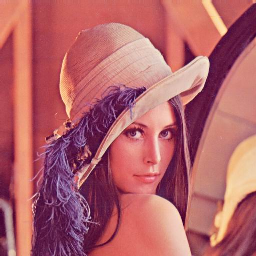
\includegraphics[width=\textwidth]{lenac_small.png}
        \caption{original}
    \end{subfigure}\\[2ex]
    \begin{subfigure}[t]{\subfiguresize}
        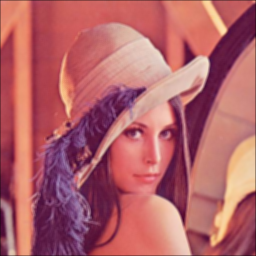
\includegraphics[width=\textwidth]{lenac_lowpass1.png}
        \caption{low-pass with mask $\mathbf{M}_1$}
    \end{subfigure}
    \begin{subfigure}[t]{\subfiguresize}
        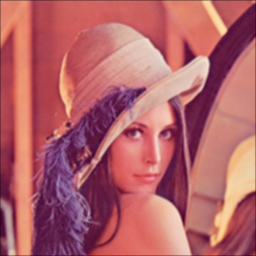
\includegraphics[width=\textwidth]{lenac_lowpass2.png}
        \caption{low-pass with mask $\mathbf{M}_2$}
    \end{subfigure}
    \begin{subfigure}[t]{\subfiguresize}
        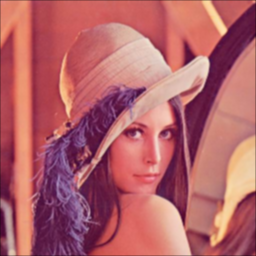
\includegraphics[width=\textwidth]{lenac_lowpass3.png}
        \caption{low-pass with mask $\mathbf{M}_3$}
    \end{subfigure}
    \caption{Results of running the low-pass filter with different masks}
    \label{fig:lowpass-results-original}
\end{figure}

As we can see, the images after filtering seem to be more blurred.
This is expected, due to the characteristic of the low-pass filter.
It attenuates the high frequencies, which in case of the images means rapid change in pixel lumininosity.
These rapid changes often occur at the edges of objects, therefore, the filtered image appears softer and less sharp.

However, since this filter is good at attenuating rapid changes in luminosity, it can be used as a way of reducing the noise in the image.
The results of such experiment are presented on fig. \ref{fig:lowpass-results-noise}.

\begin{figure}[ht]\centering
    \begin{subfigure}[t]{\subfiguresize}
        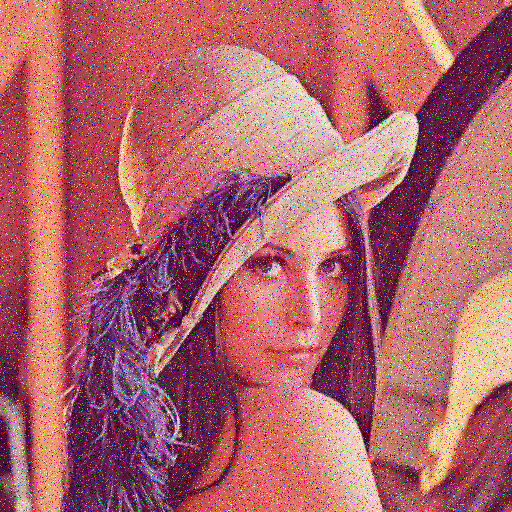
\includegraphics[width=\textwidth]{lenac_uniform3.png}
        \caption{uniform noise}
    \end{subfigure}
    \begin{subfigure}[t]{\subfiguresize}
        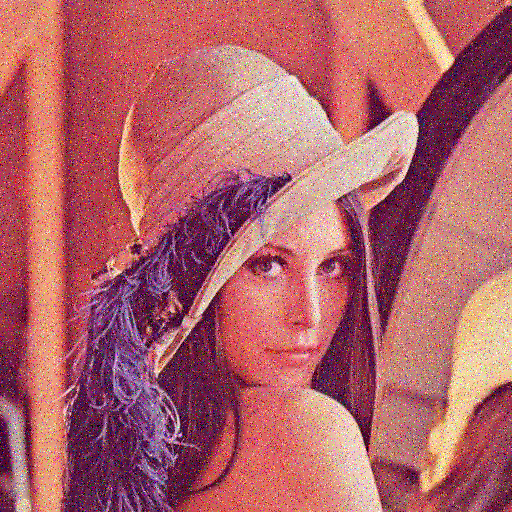
\includegraphics[width=\textwidth]{lenac_normal3.png}
        \caption{gaussian noise}
    \end{subfigure}
    \begin{subfigure}[t]{\subfiguresize}
        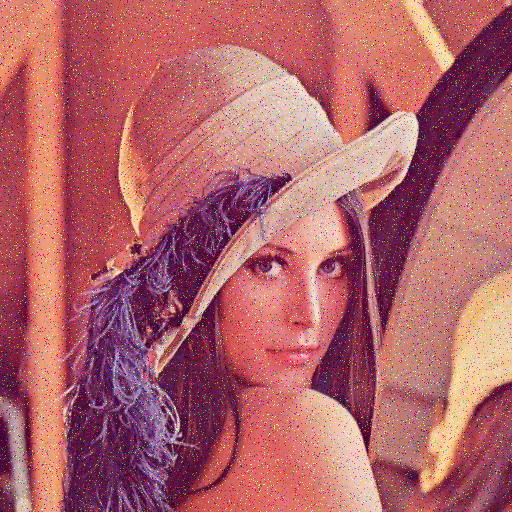
\includegraphics[width=\textwidth]{lenac_impulse3.png}
        \caption{impulse noise}
    \end{subfigure}\\[2ex]
    \begin{subfigure}[t]{\subfiguresize}
        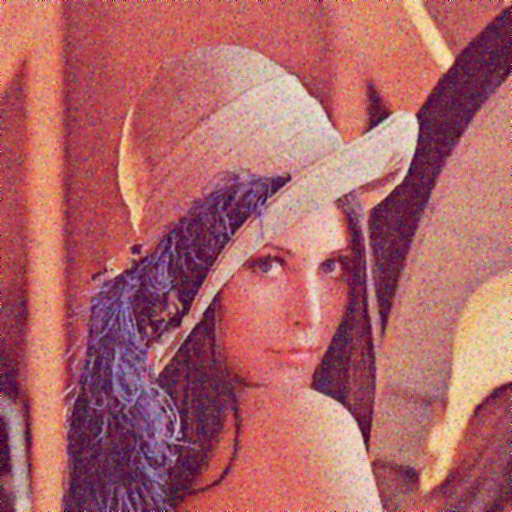
\includegraphics[width=\textwidth]{lenac_lowpass_uniform_1.png}
        \caption{filtered uniform noise}
    \end{subfigure}
    \begin{subfigure}[t]{\subfiguresize}
        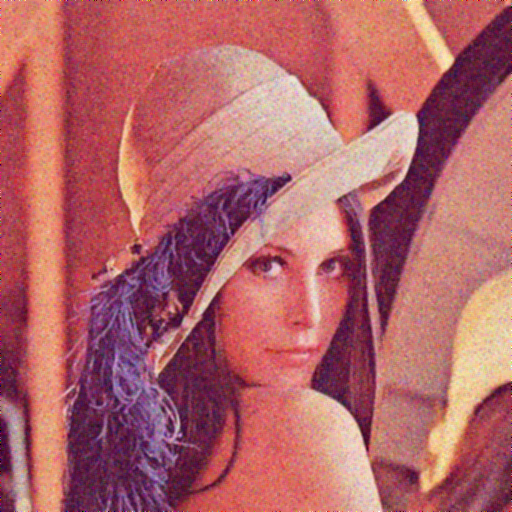
\includegraphics[width=\textwidth]{lenac_lowpass_normal_1.png}
        \caption{filtered gaussian noise}
    \end{subfigure}
    \begin{subfigure}[t]{\subfiguresize}
        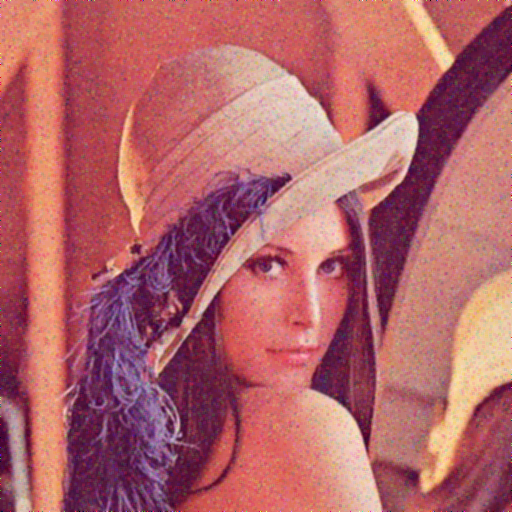
\includegraphics[width=\textwidth]{lenac_lowpass_impulse_1.png}
        \caption{filtered impulse noise}
    \end{subfigure}
    \caption{Results of running the low-pass filter with $\mathbf{M}_1$ on different noise types}
    \label{fig:lowpass-results-noise}
\end{figure}

The results are positive, although not perfect.
The filtered images still have visible grain from the noise, however, they are much softer than in the unfiltered noise.
The filter did not remove the noise, but rather blurred it, which made it stand out less.

However, to objectively veryfy if the resulting images have less noise, we compared them to the original image (without noise).
The result of this comparison is presented in table \ref*{tab:lowpass-results-noise} below.

\begin{table}[H]\centering
    \begin{tabular}{l|ccccc}
        \toprule
        image                 & \textsc{mse} & \textsc{pmse} & \textsc{snr} & \textsc{psnr} & \textsc{md} \\
        \midrule[.5pt]
        uniform noise         & 1203         & 4.72          & 8.38         & 17.33         & 152         \\
        filtered unif. noise  & 166          & 0.65          & 16.98        & 25.93         & 149         \\
        \midrule[.1pt]
        gaussian noise        & 755          & 2.96          & 10.40        & 19.35         & 79          \\
        filtered gauss. noise & 109          & 0.43          & 18.83        & 27.78         & 81          \\
        \midrule[.1pt]
        impulse noise         & 597          & 2.34          & 11.42        & 20.37         & 144         \\
        filtered imp. noise   & 91           & 0.36          & 19.61        & 28.56         & 144         \\
        \bottomrule
    \end{tabular}
    \caption{Image comparison metrics for images with noise before and after applying the low-pass filter}
    \label{tab:lowpass-results-noise}
\end{table}

We can clearly see that the filtered images are better than the unfiltered versions.


\pagebreak[3]
\section{Description of the non-linear filter implementation }

\subsection{Mathematical description}

Our task was to implement the uolis operator, which was defined as the following:
\begin{equation}
    g(x,y) = \frac{1}{4} \log \left(
    \frac{f(x,y)^4}{A_1 A_3 A_5 A_7}
    \right)
    \label{eq:uolis}
\end{equation}
where,
\begin{align*}
    A_1 & = f(x,y-1) \\
    A_3 & = f(x+1,y) \\
    A_5 & = f(x,y+1) \\
    A_7 & = f(x-1,y)
\end{align*}

Since the logaritm base was not explicitly stated, we assumed $\log_{10}$, according to standard mathematical notation.
Note that equation (\ref{eq:uolis}) can be expressed as
\begin{equation*}
    g(x,y) = \frac{1}{4} \left[
        \log\left(\frac{f(x,y)}{A_1}\right) +
        \log\left(\frac{f(x,y)}{A_3}\right) +
        \log\left(\frac{f(x,y)}{A_5}\right) +
        \log\left(\frac{f(x,y)}{A_7}\right)
        \right]
\end{equation*}
which is just the arithmetic means of the logarithms of the ratios of the horizontally and vertically neighboring pixels.
For similar pixels, the values of the logarithms will be close to 0, therefore the resulting image will be close to black.
However, if there is a drastic change in the luminosity values, the logaritm will be a positive value, resulting in a brighter pixel in the output image.

Note that for 255 discrete luminosity levels, the maximum value that the uolis operator can output is $\log_{10}(255) \approx 3$ (assuming there is no division by 0, in which case it would be $+\infty$).
This is very dim, almost not visible in the result.
That is because, the uolis operator does not take into account the representation of the pixel luminosity.
It is best suited for formats, where luminosity is stored as a floating point number in the range $\langle 0, 1 \rangle$.
Therefore, we must normalize the output to our format (integer in the range $\langle 0, 255 \rangle$), by multiplying by 255.
However, we noticed that the output is still not very visible, so we decided to multiply it by additional factor of 10, resulting in final multiplication by 2550.

Therefore, eq. (\ref{eq:uolis}) will take the final form:
\begin{equation}
    g(x,y) = 2550 \cdot \frac{1}{4} \log \left(
    \frac{f(x,y)^4}{A_1 A_3 A_5 A_7}
    \right)
    \label{eq:uolis-normalized}
\end{equation}

The comparison between results obtained from equations (\ref*{eq:uolis}) and (\ref*{eq:uolis-normalized}) is shown on fig.~\ref{fig:uolis}.

\pagebreak[3]
\subsection{Implementation}

Having the equation (\ref{eq:uolis-normalized}), implementing the operator is very straightforward.
Fistly we collect the neighboring pixels ($A_1,A_3,A_5,A_7$).
Secondly, we calculate their product, and input all the other values to the equation.
Finally, we multiply by the abovementioned normalization factor of 2550.

\begin{lstlisting}[
    basicstyle=\footnotesize\ttfamily,
    morekeywords={const}
]
const NORMALIZATION_FACTOR: f64 = 2550.0;
/* ... */
let neighbors = {
    let mut neighbors: Vec<&Rgb<u8>> = vec![];
    for (i, j) in [(-1, 0), (1, 0), (0, -1), (0, 1)] {
        let xi = (x as i32 + i) as u32;
        let yi = (y as i32 + j) as u32;
        if xi < image.width() && yi < image.height() {
            neighbors.push(image.get_pixel(xi, yi));
        }
    }
    neighbors
};
for channel in 0..3 {
    let product = neighbors.iter()
        .map(|x| x[channel] as f64)
        .product::<f64>();
    let power = (image.get_pixel(x, y)[channel] as f64).pow(4.0);
    let log = f64::log10(power / product);
    pixel[channel] = (NORMALIZATION_FACTOR * log / 4.0) as u8
}
\end{lstlisting}

For pixels on edges, some of the $A$ neighbors do not exist, therefore, we just skip the edge pixels, leaving them black.

\section{Analysis of the filtering results (non-linear filter)}
\subsection{Results}



\begin{figure}[H]\centering
    \hfill
    \begin{subfigure}[t]{\subfiguresize}
        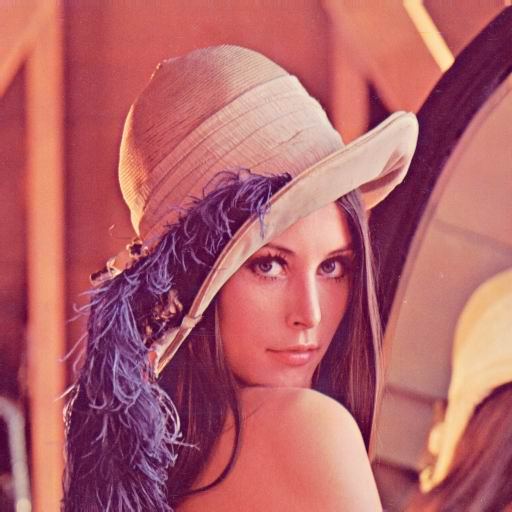
\includegraphics[width=\textwidth]{lenac.png}
        \caption{original}
    \end{subfigure}
    \hfill
    \begin{subfigure}[t]{\subfiguresize}
        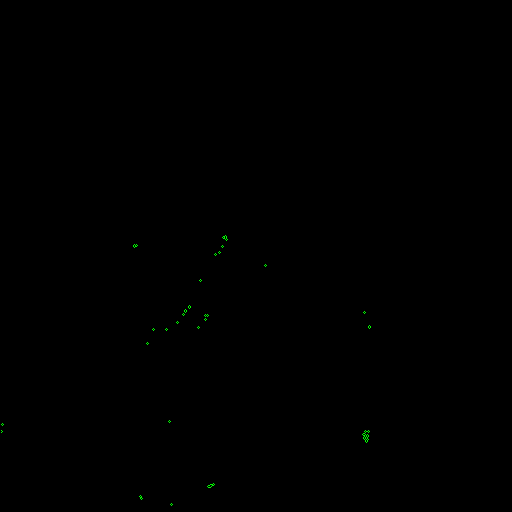
\includegraphics[width=\textwidth]{lena_uolis_clear.png}
        \caption{ordinary uolis operator}
    \end{subfigure}
    \hfill
    \begin{subfigure}[t]{\subfiguresize}
        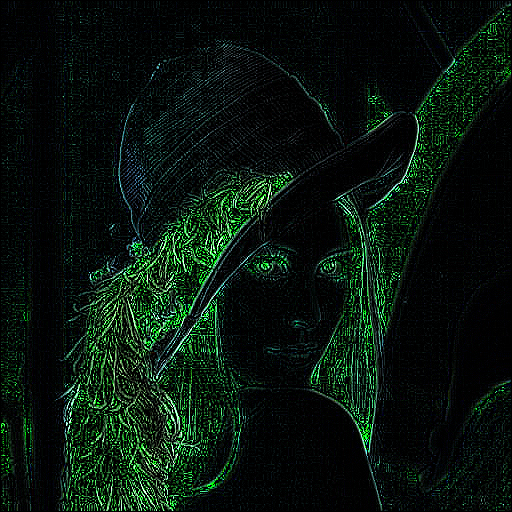
\includegraphics[width=\textwidth]{lena_uolis_normalized.png}
        \caption{normalized uolis}
    \end{subfigure}
    \hfill
    \caption{Difference between ordinary and normalized uolis operator}
    \label{fig:uolis}
\end{figure}

The results of running the uolis operator are presented on fig. \ref{fig:uolis}.
As we can see, the not normalized version is completely unreadable.
However, when we boost the output,
we can clearly see that this operator highlited the most prominent edges in the image.

\begin{figure}[H]\centering
    \begin{subfigure}[t]{\subfiguresize}
        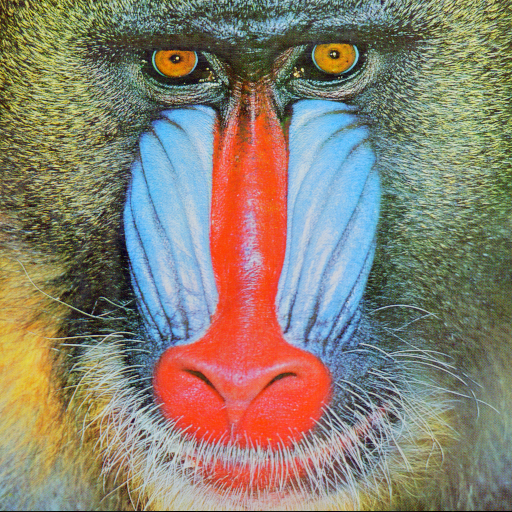
\includegraphics[width=\textwidth]{baboon.png}
        \caption{original}
    \end{subfigure}
    \hspace{1em}
    \begin{subfigure}[t]{\subfiguresize}
        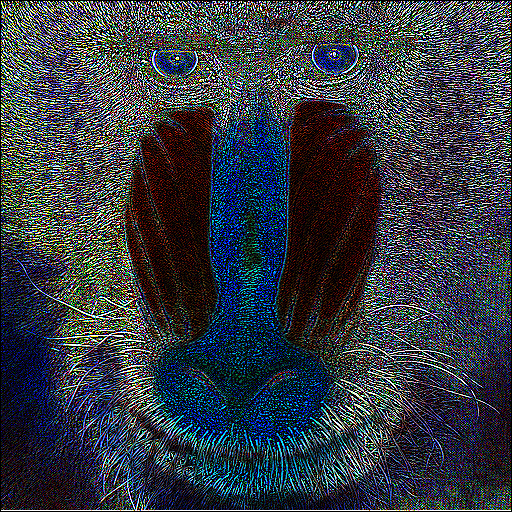
\includegraphics[width=\textwidth]{baboon_uolis.png}
        \caption{after uolis operator}
    \end{subfigure}
    \\
    \begin{subfigure}[t]{\subfiguresize}
        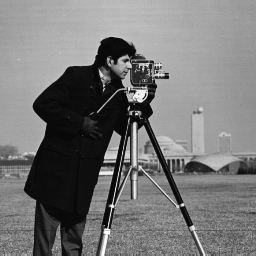
\includegraphics[width=\textwidth]{cameraman.png}
        \caption{original}
    \end{subfigure}
    \hspace{1em}
    \begin{subfigure}[t]{\subfiguresize}
        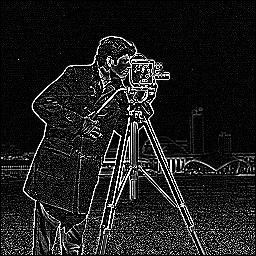
\includegraphics[width=\textwidth]{cameraman_uolis.png}
        \caption{after uolis operator}
    \end{subfigure}
    \\
    \begin{subfigure}[t]{\subfiguresize}
        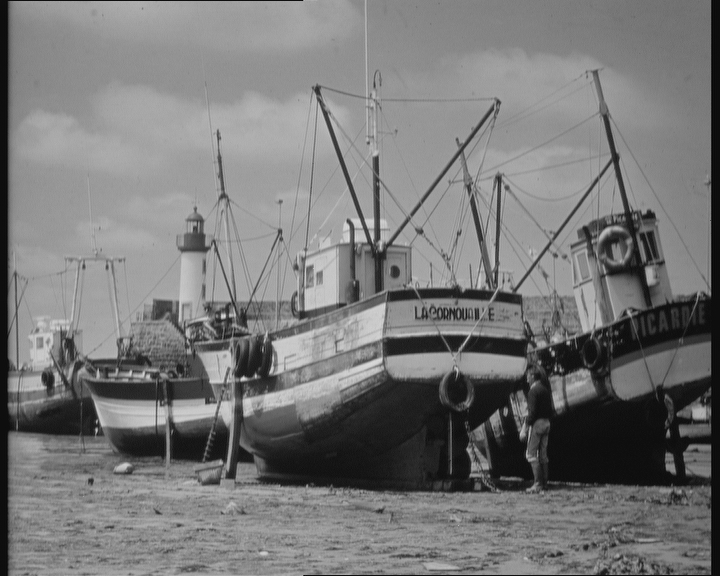
\includegraphics[width=\textwidth]{boats.png}
        \caption{original}
    \end{subfigure}
    \hspace{1em}
    \begin{subfigure}[t]{\subfiguresize}
        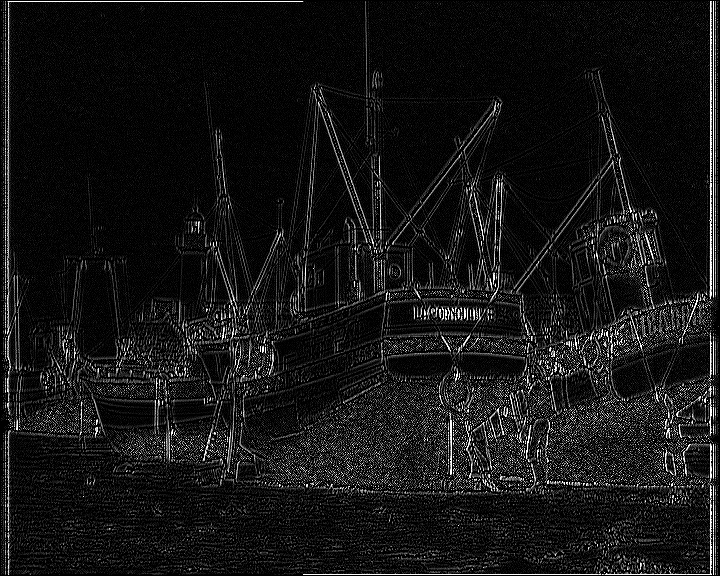
\includegraphics[width=\textwidth]{boats_uolis.png}
        \caption{after uolis operator}
    \end{subfigure}
    \caption{Results of applying uolis operator to various images}
    \label{fig:uolis-more}
\end{figure}

\section{Description of other changes which took place in the application}

The application has a big change in terms of the structure, 
we divided the monolythic project into a library responsible for image operations,
and a binary, responsible for interfacing with user via CLI.
This made the development process more easy, as the responsibilities were clearly divided and the project was easier to navigate.

Learing from previous mistakes with implementing signal to noise ration,
this time we created unit tests for our calculations in order to avoid mistakes.
Those tests quickly came to use, because of minor difficulties with mathematical equations.

\vfill
\section*{Teacher's remarks}
\begin{tabularx}{\textwidth}{|X|}
    \hline
    \vspace{7cm}
    \phantom{.} \\
    \hline
\end{tabularx}

\end{document}